\chapter{Identifikationsprotokolle} Nachdem wir jetzt Authentifikation
von Nachrichten und den authentifizierten Austausch von Schlüsseln
betrachtet haben, befasst sich dieses Kapitel mit der asymmetrischen
Identifikation von Kommunikationsteilnehmern. Das bedeutet, Alice ist im
Besitz eines geheimen Schlüssels $\skey$ und Bob, der den dazugehörigen
öffentlichen Schlüssel $\pkey$ kennt, möchte sicher sein, dass er mit
einer Instanz redet, die in Besitz von $\skey$ ist. Üblicherweise geht
es bei dieser Prüfung um den Nachweis einer Identität, der an bestimmte
(Zugangs-)Rechte gekoppelt ist.

Da Alice im Folgenden \emph{beweisen} muss, dass sie den geheimen
Schlüssel besitzt, und Bob ihre Identität \emph{überprüft}, heißen die
beiden für den Rest dieses Kapitels \texttt{Prover} und
\texttt{Verifier}.

Der einfachste Weg, dem Verifier zu beweisen, dass der Prover das
Geheimnis $\skey$ kennt, ist es, ihm den Schlüssel einfach direkt zu
schicken. Der Verifier kann dann die Zugehörigkeit zu $\pkey$
feststellen und sicher sein, dass der Prover das Geheimnis
kennt. Allerdings wird bei diesem Vorgehen $\skey$ allgemein bekannt und
garantiert nach der ersten Verwendung keine Zuordnung mehr zu einer
bestimmten Identität.

Die Protokollanforderungen steigen also darauf, dass der Verifier sicher
sein kann, dass der Prover das Geheimnis kennt, der Verifier selbst
jedoch $\skey$ nicht lernt.

Ein zweiter Versuch umfasst die bereits entwickelten
Signaturschemata. Der Prover schickt $\sigma := \sig(\skey_A,
\text{"`ich bin's, P"'})$ an den Verifier.  $\ver(\pkey_A,\text{"`ich
bin's, P"'}, \sigma)$ liefert dem Verifier die Gültigkeit der
entsprechenden Signatur und damit die Identität des Absenders. Die Idee
hierbei ist, dass der Angreifer eine Signatur fälschen müsste, um das
Identifikationsprotokoll zu brechen, was ein Widerspruch zur Sicherheit
des Signaturverfahrens darstellen würde. Leider funktioniert diese
Argumentation nicht. Ein Angreifer auf das Identifikationsprotokoll
könnte eine bereits gesehene Signatur $\sigma$ wiederverwenden, um sich
gegenüber anderen als den Prover P auszugeben. Dies kann er
beispielsweise in einem Man-in-the-Middle-Angriff oder einer
Replay-Attacke tun.

Aus den ersten beiden Versuchen geht hervor, dass wir ein interaktives
Protokoll wie in Abbildung \ref{fig:id:interaktiv} benötigen, um den
geheimen Schlüssel gleichzeitig zu verbergen und den Besitz dieses
Geheimnisses zu beweisen. Die Sicherheit eines solchen Verfahrens wird
in Kapitel \ref{sec:id:protokolle} näher betrachtet.

\begin{figure}[h]
\begin{center} \unitlength=1mm \linethickness{0.4pt} \hspace{-3 cm}
\begin{picture}(30,20)
\put(10,15){\makebox(0,0)[cb]{$\mathtt{Prover}_{\skey_A}$}}
\put(50,15){\makebox(0,0)[cb]{$\mathtt{Verifier}_{\pkey_A}$}}
    
    \put(10,0){\line(0,1){13}} \put(50,0){\line(0,1){13}}

    \put(50,10){\vector(-1,0){40}} \put(30,11){\makebox(0,0)[cb]{$R$}}
    
    \put(10,3){\vector(1,0){40}} \put(30,4){\makebox(0,0)[cb]{$\sigma :=
\sig(\skey_A, R)$}}
\end{picture}
\end{center}
\caption[foobar]{Interaktives Protokoll, in dem der Verifier dem Prover eine
Zufallszahl $R$ gibt, um dessen Identität durch eine Signatur
sicherzustellen \footnote{Es kann sinnvoll sein,
nicht nur die Zufallszahl $R$ zu signieren, sondern dieser noch das
aktuelle Datum und die aktuelle Uhrzeit hinzuzufügen. So kann, selbst
wenn der Verifier irgendwann zum zweiten Mal die selbe Zufallszahl
ausgibt, eine gerade erzeugte von einer alten Signatur unterschieden
werden.}.}
\label{fig:id:interaktiv}
\end{figure}

\section{Sicherheitsmodell}
\begin{definition}[Public-Key-Identifikationsprotokoll]
Um ein Sicherheitsmodell zu Identifikationsprotokollen betrachten zu
können, definieren wir uns ein solches zunächst formal.
\end{definition}
\begin{definition}
Ein \textit{Public-Key-Identifikationsprotokoll} ist definiert durch ein 3-Tupel
$(\gen, \mathrm{P}, \mathrm{V})$ von PPT-Algorithmen. Dabei gibt $\gen$
wie gewohnt bei Eingabe eines Sicherheitsparameters $1^k$ das
Schlüsselpaar $(\pkey, \skey)$ aus. Der Prover P und der Verifier V sind
zustandsbehaftet und interagieren während des Identitätsnachweises
miteinander.
\end{definition}

Der Ablauf eines solchen Protokolls läuft folgendermaßen ab:
\begin{enumerate}
  \item V erhält den öffentlichen Schlüssel $\pkey$ als Eingabe und
gibt $\mathrm{out}_V$ aus.
  \item P erhält Vs Ausgabe $\mathrm{out}_V$ und gibt $\mathrm{out}_P$ aus.
  \item V erhält Ps Ausgabe $\mathrm{out}_P$ und gibt $\mathrm{out}_V$
    aus.
  \item ist $\mathrm{out}_V \in \{0,1\}$ beende die Interaktion,
    ansonsten springe zurück zu Schritt 2.
\end{enumerate} 

  
\begin{figure}
\begin{center}
    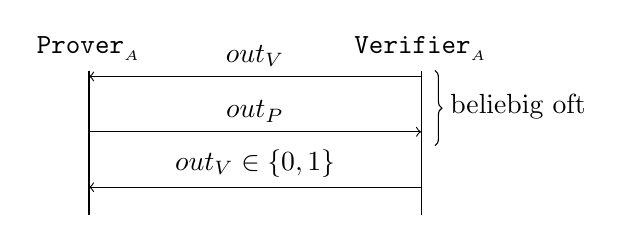
\begin{tikzpicture}[x=1em, y=1em]
      \draw (-6,0) node (P) {$\mathtt{Prover}_{\skey_A}$}; 
      \draw (6,0) node (V) {$\mathtt{Verifier}_{\pkey_A}$};
      
      \draw (P) -- (-6,-6);
      \draw (V) -- (6,-6);
      
      \draw[->] (6 ,-1) -- (-6, -1)
        node[sloped,above, pos=0.5] {$out_{V}$}; 
      
      \draw[->] (-6 ,-3) -- (6, -3)
        node[sloped,above, pos=0.5] {$out_{P}$}; 
      
      \draw[decoration={brace,raise=5pt},decorate] (V) --(6,-3.5)
        node[above, pos=0.77, xshift=35]{beliebig oft} (6, -3.5);

      \draw[->] (6 ,-5) -- (-6, -5)
        node[sloped,above, pos=0.5] {$out_V \in \{0, 1\}$}; 
      
    \end{tikzpicture}
  \caption{Ablauf eines Public-Key-Identifikationsprotokolls}
  \label{fig:pki-identifikation}
\end{center}
\end{figure}


Der Verifier erzeugt also eine Ausgabe, mit deren Hilfe
P beweisen muss, dass er das Geheimnis $\skey$ kennt. P liefert auf Basis
des Geheimnisses und der Ausgabe von V seinerseits eine Ausgabe und gibt
diese an V weiter. Möglicherweise tauschen P und V mehrmals wie eben
beschrieben Nachrichten aus. Am Ende prüft V das Ergebnis und
entscheidet, ob die Idendtifikation erfolgreich abgeschlossen wurde. Falls ja,
gibt er 1 aus, falls nein 0. 

% Das Verfahren muss \emph{korrekt} sein, also muss schließlich gelten:
% \begin{align*}
%  \forall (\pkey, \skey) \leftarrow \gen(1^k):
% V(\mathrm{out}_P) \rightarrow 1
% \end{align*}
Das Verfahren muss \emph{korrekt} sein, d.h für alle $(\pkey, \skey)
\leftarrow \gen(1^k)$ wird $V$ am Ende des interaktiven Protokolls mit
$P$ $1$ ausgeben. 
%  $\langle \mathrm{P}(\skey), \mathrm{V}(\pkey) \rangle$
% bezeichnet im Folgenden das Transkript der Interaktion zwischen Prover
% und Verifier.

Einem Angreifer $\A$ darf es nun intuitiv nicht möglich sein, gegenüber
einem Verifier die Identität eines anderen Provers anzunehmen. Um das zu
präzisieren, führen wir ein neues Spiel ein. Zunächst erzeugt der Challenger $i$
$(\pkey, \skey)$-Paare mithilfe des $\gen$-Algorithmus und ordnet die privaten Schlüssel $i$ Provern zu.
\begin{enumerate}
  \item $\A$ darf nun mit beliebig vielen dieser gültigen Prover
interagieren. Dabei nimmt er die Rolle des Verifiers ein und hat demnach
Zugriff auf die passenden öffentlichen Schlüssel $\pkey_i$, während die
gültigen Prover seine Anfragen mit ihren privaten Schlüsseln $\skey_i$
beantworten.
  \item $\A$ wählt sich nun einen der $\pkey_{i}$ aus und gibt sich
    damit gegenüber dem Challenger (welcher nun als \glqq echter\grqq
    Verifier fungiert) als Prover $i$ aus. der Challenger erhält als
    Eingabe $\pkey_i$ von \A.
  \item $\A$ gewinnt, wenn der Challenger als Ergebnis schließlich 1
ausgibt.
\end{enumerate} Wir nennen ein Public-Key-Identifikationsprotokoll
$(\gen, \mathrm{P}, \mathrm{V})$ sicher, wenn kein PPT-Angreifer $\A$
das oben genannte Spiel häufiger als vernachlässigbar oft gewinnt.

Allerdings verhindert das oben genannte Spiel keinen
Man-in-the-Middle-Angriff, in dem $\A$ die Ausgaben einfach
weiterreicht.


\section{Protokolle}\label{sec:id:protokolle}
Mithilfe des eben definierten Sicherheitsbegriffs können wir nun die
Sicherheit des Vorschlags aus Abbildung \ref{fig:id:interaktiv} genauer untersuchen.
Dieser Ansatz basiert auf einem Signaturverfahren. Seine
Sicherheit ist demnach von der Sicherheit des verwendeten
Signaturalgorithmus abhängig.~\\

\begin{theorem} Ist das verwendete Signaturverfahren EUF-CMA-sicher, so
ist das in Abbildung \ref{fig:id:interaktiv} gezeigte
PK-Identifikationsprotokoll $(\gen, \mathrm{P}, \mathrm{V})$ sicher.~\\
\end{theorem}
\begin{beweisidee} Angenommen, es gibt einen Angreifer $A$, der das
PK-Identifikationsprotokoll bricht. Dann ist er in der Lage,
nicht-vernachlässigbar oft aus dem öffentlichen Schlüssel $\pkey_{i^*}$
und einer vom Verifier ausgewählten Zufallszahl $R$ eine Signatur
$\sigma := \sig(\skey_{i^*}, R)$ zu berechnen.

Aus $A$ kann nun ein Angreifer $B$ konstruiert werden, der die
Ergebnisse von $A$ nutzt, um das EUF-CMA-sichere Signaturverfahren zu
brechen.~\\
\end{beweisidee}

Ein weiterer Ansatz für ein funktionierendes Identifikationsprotokoll
auf Public-Key-Basis ist in Abbildung \ref{fig:id:protokoll2}
dargestellt.  Hier wird $R$ vor der Übertragung über die Leitung vom
Verifier mit $\pkey_{i^*}$ verschlüsselt, sodass die Kenntnis von
$\skey_{i^*}$ durch einen Entschlüsselungsvorgang überprüft wird.

Es ist hierbei darauf zu achten, dass das Schlüsselpaar, das für dieses
Identifikationsprotokoll verwendet wird, nicht auch zum Verschlüsseln
gebraucht werden sollte. Ansonsten kann ein Angreifer in der Rolle des
Verifiers die Entschlüsselung von ihm bekannten Chiffraten herbeiführen
und somit jedes beliebige Chiffrat entschlüsseln lassen.

\begin{figure}[h]
\begin{center} \unitlength=1mm \linethickness{0.4pt} \hspace{-3 cm}
    \begin{picture}(50,30)(0,0)
\put(10,22){\makebox(0,0)[cb]{\texttt{Prover}$_{\skey_{i^*}}$}}
\put(10,0){\line(0,1){20}}
    
        \put(70,22){\makebox(0,0)[cb]{\texttt{Verifier}$_{\pkey_{i^*}}$}}
\put(70,0){\line(0,1){20}}
        
        \put(40,16){\makebox(0,0)[cb]{$\ciphert \leftarrow
\enc(\pkey_{i^*}, R)$}} \put(70,15){\vector(-1,0){60}}
        
        \put(40,6){\makebox(0,0)[cb]{$R = \dec(\skey_{i^*}, \ciphert)$}}
\put(10,5){\vector(1,0){60}}
    \end{picture}
\end{center}
\caption{Dieses Identifikationsprotokoll profitiert von der Sicherheit
des verwendeten Public-Key-Verschlüsselungsverfahrens.}
\label{fig:id:protokoll2}
\end{figure}



\begin{theorem} Ist das in Abbildung \ref{fig:id:protokoll2} verwendete
Verschlüsselungsverfahren IND-CCA-sicher, so ist das darauf basierende
PK-Identifikationsprotokoll $(\gen, \mathrm{P}, \mathrm{V})$ sicher.
\end{theorem}

\begin{beweisidee} Der Beweis dafür läuft analog zum obigen. Aus einem
Angreifer $A$, der das Identifikationsprotokoll nicht vernachlässigbar
oft bricht, wird ein Angreifer $B$ konstruiert, der das IND-CCA-sichere
Verschlüsselungsverfahren bricht.
\end{beweisidee}

Identifikationsprotokolle wie die in Abbildungen \ref{fig:id:interaktiv}
und \ref{fig:id:protokoll2} gezeigten heißen auch
"`Challenge-Response-Verfahren"', denn der Verifier stellt dem Prover
eine Aufgabe (oder Herausforderung, die "`Challenge"'), die nur der
echte Prover lösen kann. In dem Protokoll aus Abbildung
\ref{fig:id:interaktiv} ist diese Aufgabe die Erstellung einer Signatur
für einen Zufallsstring~$R$; in Abbildung \ref{fig:id:protokoll2} ist
diese Aufgabe die Entschlüsselung eines zufälligen Chiffrats $C =
\enc(\pkey_{i^*}, R)$. Die Lösung des Provers wird daher auch als die
Antwort, oder "`Response"' bezeichnet.
